\documentclass [a4paper] {article}

\usepackage[utf8]{inputenc}

\title{Practica 6: Fundamentos de la Ciencia de Datos}
\author{
  Daniel López Moreno\\
  \and
  Alejandro Fernández Maceira\\
  \and
  Álvaro Maestre Santa
}

\usepackage{Sweave}
\begin{document}

\maketitle

\section{Mapa Coroplético}

En esta práctica se nos pide,que desarrollemos con toda la profundidad posible un tipo de 
gráfico de visualización de datos. En nuestro caso hemos optado por un tipo de gráfico
denominado \textbf{Mapa Coroplético}.

\subsection{¿Qué es un mapa coroplético?}

Un mapa coroplético es un tipo de gráfico que muestra una determinada \textbf{región geográfica dividida 
en distintas secciones}. Sobre nuestro mapa se \textbf{mide una variable} en concreto y posteriormente
cada una de las secciones del mapa se \textbf{colorea} con un \textbf{tono más claro o más oscuro} en función de la
frecuencia absoluta o relativa de la variable en dicha sección.

\begin{center}
  \centering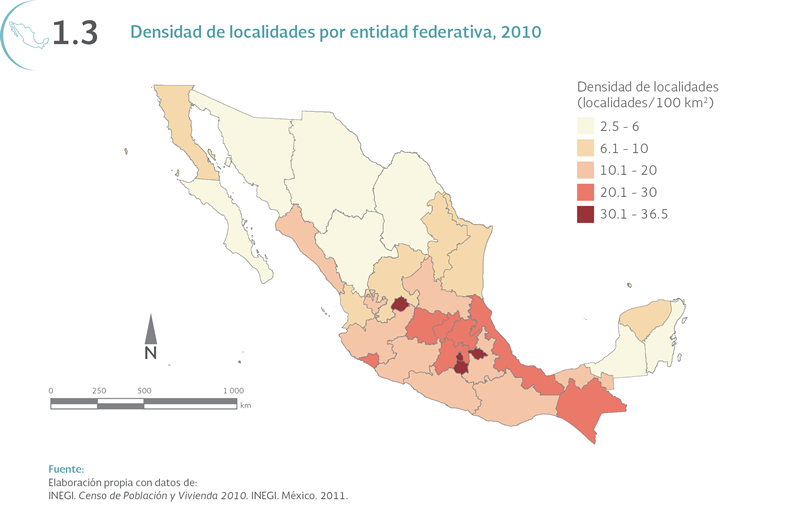
\includegraphics{mapacloropletico.png}
  \\\textbf{Figura 1}: Ejemplo de mapa cloroplético 
\end{center}


Este tipo de gráfico suele estar compuesto por los siguientes elementos:
\begin{itemize} 
  \item \textbf{Mapa}: El elemento principal de este gráfico es el mapa situado en el centro, dividido en distintas
  regiones.
  \item \textbf{Leyenda}: Todos los mapas coropléticos incluyen una leyenda que nos indica los distintos rangos de 
  la variable a medir junto a un gradiente de color de más claro a más oscuro.
  \item \textbf{Título}: Todo mapa cloroplético debe incluir un título que nos indique que se está representando en
  nuestro gráfico.
\end{itemize}

\subsubsection{Ventajas de un mapa coroplético}

Un mapa coroplético resulta muy útil en determinadas ocasiones ya que es un tipo de gráfico muy \textbf{fácil de entender}.
Además, es muy fácil localizar las zonas donde encontramos \textbf{máximos o mínimos} en los datos ya que suele resultar sencillo
encontrar las secciones con un color más oscuro o más claro.

\subsubsection{Desventajas de un mapa coroplético}

Una de las desventajas de este tipo de gráficos es que a veces puede resultar \textbf{difícil distinguir en que rango de color}
se encuentra una determinada sección si se encuentra en uno de los rangos intermedios de la progresión de color.
Otra desventaja que podriamos destacar es que como los datos se dividen en rangos, es más \textbf{dificil obtener información
exacta} a través de los colores.

\subsection{Desarrollo de un mapa coroplético en R}

\subsubsection{Mapa sobre votos en EEUU}
En este ejemplo vamos a realizar un mapa coroplético sobre el \textbf{porcentaje de votos a George Bush en las elecciones de Estados
Unidos de 2004}.
Comenzaremos a desarrollar nuestro propio gráfico de mapa coroplético. Para ello utilizaremos
las siguientes librerias:

\begin{Schunk}
\begin{Sinput}
> install.packages("RColorBrewer")
> install.packages("rgdal")
> library(RColorBrewer)
> library(rgdal)
\end{Sinput}
\end{Schunk}

Ahora cargaremos nuestro \textbf{shapefile} en el workspace para trabajar con él:

\begin{Schunk}
\begin{Sinput}
> USvotos <- readOGR(dsn="Shapefile", layer = "2004_Election_Counties")
\end{Sinput}
\end{Schunk}

\begin{itemize} 
  \item \textbf{Dsn}: Con dsn especificamos el directorio en el que se encuentra nuestro shapefile, en nuestro caso pondremos
  un punto "." ya que el archivo está en el mismo directorio de trabajo .
  \item \textbf{Layer}: En el atributo layer especificaremos el nombre de nuestro shapefile que vamos a cargar.
\end{itemize}

A continuación elegiremos nuestra paleta de colores. Tenemos distintas paletas de colores gracias al paquete \textbf{RcolorBrewer}:

\begin{center}
\begin{Schunk}
\begin{Sinput}
> display.brewer.all()
\end{Sinput}
\end{Schunk}
\includegraphics{memoria6-003}
\\\textbf{Figura 2}: Todas las paletas de colores disponibles.
\end{center}

Para nuestro ejemplo utilizaremos la paleta de colores \textit{Reds}:

\begin{Schunk}
\begin{Sinput}
> paleta <- brewer.pal(8, "Reds")
\end{Sinput}
\end{Schunk}

Ahora indicaremos los intervalos de nuestros votos y separaremos los datos de cada condado asignandolos según el rango de 
porcentaje al que pertenezcan:

\begin{Schunk}
\begin{Sinput}
> rangos <- c(0, 20, 40, 50, 60, 80, 100)
> cut(USvotos$Bush_pct, rangos)
> esquema_color <- paleta[findInterval(USvotos$Bush_pct, vec = rangos)]
\end{Sinput}
\end{Schunk}

Con la función \textbf{cut} separamos la columna correspondiente al porcentaje de votos de bush en los distintos rangos
especificados en la variable \textbf{rangos}.
Posteriormente en función de la paleta que hayamos escogido asignamos a la variable \textbf{esquema\_color} el mapa ya coloreado
por condados según su pertenencia a un rango o a otro.

Por último generamos el gráfico y añadimos una leyenda:

\begin{center}
\begin{Schunk}
\begin{Sinput}
> plot(USvotos, col = esquema_color,
+ main = "Porcentaje de votos para Bush - 2004", cex = 5)
> legend(-119, 31.5, legend = levels(cut(USvotos$Bush_pct, rangos)),
+ fill = esquema_color, cex = 0.8, title = "% vote for Bush")
\end{Sinput}
\end{Schunk}
\includegraphics{memoria6-006}
\\\textbf{Figura 3}: Mapa coroplético de votos a Bush en 2004.
\end{center}

En cuanto a la función \textbf{plot} tenemos los siguientes parámetros:
\begin{itemize} 
  \item \textbf{USvotos}: Datos sobre los que vamos a realizar la gráfica.
  \item \textbf{Col}: Este atributo sirve para especificar el color de nuestro gráfico, en nuestro caso será la variable esquema\_color 
  que hemos creado anteriormente.
  \item \textbf{Main}: Título de nuestro gráfico.
  \item \textbf{Cex}: Este parámetro indica la escala del texto.
\end{itemize}

En cuanto a la función \textbf{legend} tenemos los siguientes parámetros:
\begin{itemize} 
  \item \textbf{x}: Coordenada x de posicionamiento de nuestra leyenda, en nuestro caso \textbf{-119}.
  \item \textbf{y}: Coordenada y de posicionamiento de nuestra leyenda, en nuestro caso \textbf{31.5}.
  \item \textbf{legend}: Datos que vamos a introducir en nuestra leyenda, separados en rangos.
  \item \textbf{fill}: Este parámetro se utiliza para generar cajas rellenas por distintos colores, en nuestro caso, los 
  pertenecientes a la paleta \textit{"Reds"}.
  \item \textbf{cex}: Este parámetro indica la escala del texto.
  \item \textbf{title}: Título para nuestra leyenda.
\end{itemize}

\subsubsection{Mapa sobre los intercambios Erasmus en los diferentes paises de la Unión Europea}
\textbf{Cargar Datos:}\\
Gracias a la carta de los derechos fundamentales, que nos permite el acceso a documentos de la
UE, entró en vigor en 2009, y es por ello que podemos elaborar este mapa.

En primer lugar vamos a cargar los datos de la base de datos, como el archivo es .csv nos 
facilitará a la hora de cargar los datos. Con la librería \textbf{"rio"}, podremos 
importar el conjunto de datos del archivo .csv a R. En este caso, nos vamos a remontar al
conjunto de datos del 2012-2013.

\begin{Schunk}
\begin{Sinput}
> rm(list = ls())
> install.packages("rio")
> library(rio) 
> erasmus <- import("Erasmus.csv") 
\end{Sinput}
\end{Schunk}

Lo primero que nos tenemos que dar cuenta, es que el conjunto de datos es muy grande, ya que
tiene 267.547 observaciones de 34 variables cada una. Por lo tanto, nos debería bastar para
realizar un análisis correcto.\\

\textbf{Limpieza de datos:}\\
Ahora hay que ver que datos nos interesan, para realiar este análisis, para ello, tendremos que
hacer una limpieza de datos y crear una nueva métrica. Las variables que nos interesan son 
\textbf{los códigos de país de la institución anfitriona y de la institución de origen}.
También tendremos que borrar aquello valores que faltan o no son válidos. Después de hacer
todo esto, crearemos dos vectores (erasmushome y erasmushost).

\begin{Schunk}
\begin{Sinput}
> erasmus= erasmus[!erasmus$HOST_INSTITUTION_COUNTRY_CDE == "???",]
> erasmushome=erasmus[, 4]
> erasmushost=erasmus[, 13]
\end{Sinput}
\end{Schunk}

Ahora tenemos una larga lista con los diferentes códigos de cada país. Esta información debe de
ser agregada de alguna manera, y esto lo haremos con el comando \textbf{table()}. Por lo tanto,
crearemos una matriz llamada \textbf{home}, la cual contendrá el código de cada país.

\begin{Schunk}
\begin{Sinput}
> home <- as.matrix(table(erasmushome))
> home
\end{Sinput}
\begin{Soutput}
      [,1]
AT    4602
BEFR  2683
BENL  3646
BG    1521
CH    2589
CY     286
CZ    6185
DE   28887
DK    2565
EE     789
ES   33548
FI    4258
FR   26740
GR    3325
HR     882
HU    3351
IE    1976
IS     239
IT   21411
LI      23
LT    2470
LU     400
LV    1399
MT     141
NL    6853
NO    1604
PL   11960
PT    5449
RO    3212
SE    3275
SI    1316
SK    2443
TR   12344
UK    9642
\end{Soutput}
\end{Schunk}

Ahora tenemos un problema, y es que Bélgica se divide en varias regiones: BEFR, BENL y BEDE, 
pero a parte, no es solo este problema, sino que varios estudiantes tienen BEDE(Bélgica de
habla alemana) como su código de país anfitrión, ninguno lo tiene como su código de país de
origen. Esto lo arreglamos usando la función \textbf{rbind()}, ya que podemos enlazar nuestra
tabla con una nueva observación para Bélgica en su conjunto. También podemos cambiar el nombre 
de la fila en cuestión (BE), ordenar la matriz alfabéticamente y eliminar las dos filas belgas
regionales.

\begin{Schunk}
\begin{Sinput}
> home <- rbind(home, matrix(home[2] + home[3]))
> rownames(home)[35] = "BE"
> home <- home[order(rownames(home)), ]
> home <- home[-c(3, 4)]
\end{Sinput}
\end{Schunk}

Ahora hacemos el mismo procedimiento para el anfitrión (host).

\begin{Schunk}
\begin{Sinput}
> host <- as.matrix(table(erasmushost))
> host <- rbind(host, matrix(host[2] + host[3] + host[4]))
> rownames(host)[36] = "BE"
> host <- host[order(rownames(host)), ]
> host <- host[-c(3, 4, 5)]
\end{Sinput}
\end{Schunk}

A continuación, nos podemos fijar, como tenemos variables de la misma longitud. Por lo tanto,
con el comando \textbf{cbind()}, podemos unirlos en un nuevo conjunto de datos de la siguiente
manera:

\begin{Schunk}
\begin{Sinput}
> big <- as.data.frame(cbind(home, host))
\end{Sinput}
\end{Schunk}

\textbf{Resumen:} ¿Qué tenemos ahora? tenemos un conjunto de datos con dos variables y 33
observaciones. La variable \textbf{home} nos dice cuántos ciudadanos abandonaron el país y la variable 
\textbf{host}, nos dice cuantos estudiantes extranjeros entraron en el país. Entonces, lo que
queremos es hacer una métrica que pueda comparar estas dos cifras. Básicamente es responder
la siguiente pregunta: \textbf{¿Cuántos estudiantes extranjeros se alojan por cada estudiante enviado
al extranjero?}
Por lo tanto, tenemos que crear una nueva variable en nuestro conjunto de datos formado:

\begin{Schunk}
\begin{Sinput}
> big$rat <- big$host / big$home
\end{Sinput}
\end{Schunk}

Dado que queremos crear un mapa, vamos a querer que nuestros nombres de fila (países) sean idénticos
a los nombres de fila de datos de mapa del paquete \textbf{maps}. Por lo tanto, vamos a cambiar
nuestros códigos de país en nombres de países completos. Esto lo conseguiremos, utilizando
el paquete \textbf{countrycode}, que se encargará de hacer todo esto. El comando \textbf{countrycode()}
especifica los códigos de país de Eurostat y los nombres de país como origen y destino respectivamente.
El problema, es que hay veces que falla este comando, pero se puede introducir manualmente.

\begin{Schunk}
\begin{Sinput}
> install.packages("countrycode")
> library(countrycode)
> countries <- countrycode(rownames(big), "eurostat", "eurostat.name")
> countries[13] <- "Greece"
> countries[7] <- "Germany"
> countries[33] <- "UK"
> rownames(big) <- countries
\end{Sinput}
\end{Schunk}

Ahora, el problema es que el paquete \textbf{maps}, hace referencia a países en una columna
distinta, no a las filas. Por lo tanto, vamos a copiar los nombres de fila en una nueva columan 
llamada \textbf{region}. Vamos a reordenar tambíen las oclumans para que esta columna aparezca
primero.

\begin{Schunk}
\begin{Sinput}
> big$region <- rownames(big)
> big <- big[, c(4, 1, 2, 3)]
> big
\end{Sinput}
\begin{Soutput}
                       region  home  host       rat
Austria               Austria  4602  5007 1.0880052
Belgium               Belgium  6329  6414 1.0134302
Bulgaria             Bulgaria  1521   665 0.4372124
Switzerland       Switzerland  2589  2717 1.0494399
Cyprus                 Cyprus   286   545 1.9055944
Czech Republic Czech Republic  6185  5533 0.8945837
Germany               Germany 28887 22728 0.7867899
Denmark               Denmark  2565  5632 2.1957115
Estonia               Estonia   789  1072 1.3586819
Spain                   Spain 33548 31360 0.9347800
Finland               Finland  4258  6558 1.5401597
France                 France 26740 23970 0.8964099
Greece                 Greece  3325  1467 0.4412030
Croatia               Croatia   882   533 0.6043084
Hungary               Hungary  3351  3656 1.0910176
Ireland               Ireland  1976  4644 2.3502024
Iceland               Iceland   239   493 2.0627615
Italy                   Italy 21411 16878 0.7882864
Liechtenstein   Liechtenstein    23    39 1.6956522
Lithuania           Lithuania  2470  1980 0.8016194
Luxembourg         Luxembourg   400    93 0.2325000
Latvia                 Latvia  1399   919 0.6568978
Malta                   Malta   141   492 3.4893617
Netherlands       Netherlands  6853  8445 1.2323070
Norway                 Norway  1604  4050 2.5249377
Poland                 Poland 11960  9836 0.8224080
Portugal             Portugal  5449  8696 1.5958892
Romania               Romania  3212  1649 0.5133873
Sweden                 Sweden  3275  9711 2.9651908
Slovenia             Slovenia  1316  1681 1.2773556
Slovakia             Slovakia  2443  1214 0.4969300
Turkey                 Turkey 12344  5254 0.4256319
UK                         UK  9642 18083 1.8754408
\end{Soutput}
\end{Schunk}

\textbf{Crear el mapa:}\\
Ahora vamos a crear el mapa, para ello, vamos a cargar el paquete \textbf{maps}, ya que
nos proporciona coordenadas que luego podemos trazar como polígonos para crear el mapa.
Si queremos una escala de color elegante que corresponda a nuestra métrica, vamos a tener 
que combinar parte del conjunto de datos del paquete \textbf{maps} con nuestro propio 
conjunto de datos. Por eso necesitamos que los nombres de los países correspondan con los 
nombres del conjunto de datos del paquete \textbf{maps}. Otra librería que utilizaremos será
\textbf{ggplot2}, el cual, nos dibujará el mapa. Si queremos mostrar otros países que no 
correspondan con la UE, deberemos de rellenarlos con valores "NA". Por lo tanto, necesitaremos
una lista de todas las regiones a partir de los datos del \textbf{mundo} de los \textbf{mapas},
y necesitaremos también un conjunto de datos más grande con valores NA para todos los países que
no participan en el Erasmus. Vamos a crear un conjunto de datos con nuestros datos de mapa 
\textbf{mundo}.

\begin{Schunk}
\begin{Sinput}
> install.packages("maps")
> install.packages("ggmap")
> library(maps)
> library(ggmap)
> mundo <- map_data("world")
\end{Sinput}
\end{Schunk}

A continuación, vamos a crear un marco de datos con valores "NA" para empezar, que más adelante
podemos reemplazar con nuestros valores para la métrica. Por lo tanto, queremos que tenga el 
mismo número de filas que el número de regiones del conjunto de datos \textbf{mundo}. Hay que
recordar, que nuestro objetivo es mantener nuestros valores para los países Erasmus, pero
también queremos valores "NA" para otras regiones en el conjunto de datos \textbf{mundo}, de
lo contrario estos países tendrán el mismo color que el fondo en nuestro mapa. También vamos
a crear una nueva columna con todos los nombres de región. Esto hace posible la fusión en la variable
\textbf{region}.

\begin{Schunk}
\begin{Sinput}
> tojoin <- as.data.frame(matrix(
+           nrow = length(table(mundo$region)),
+           ncol = 4,
+           NA,
+           dimnames = list(names(table(mundo$region)), colnames(big))
+   ))
> tojoin$region <- rownames(tojoin)
\end{Sinput}
\end{Schunk}

Ahora, vamos a unir a nuestros datos Erasmus con estos nombres de región y posteriormente, lo
ordenaremos el conjunto de datos resultante. \textbf{fulljoin()} nos vendrá muy bien para empezar,
ya que mantendrá todas las filas de ambas variables pero se fusionará en aquellas columnas,
que sean idénticas.

\begin{Schunk}
\begin{Sinput}
> install.packages("dplyr")
> library(dplyr)
> all <- full_join(big, tojoin)
> all <- all[order(all$region), ]
> all
\end{Sinput}
\begin{Soutput}
                                 region  home  host  rat
34                          Afghanistan    NA    NA   NA
35                              Albania    NA    NA   NA
36                              Algeria    NA    NA   NA
37                       American Samoa    NA    NA   NA
38                              Andorra    NA    NA   NA
39                               Angola    NA    NA   NA
40                             Anguilla    NA    NA   NA
41                           Antarctica    NA    NA   NA
42                              Antigua    NA    NA   NA
43                            Argentina    NA    NA   NA
44                              Armenia    NA    NA   NA
45                                Aruba    NA    NA   NA
46                     Ascension Island    NA    NA   NA
47                            Australia    NA    NA   NA
1                               Austria  4602  5007 TRUE
48                              Austria    NA    NA   NA
49                           Azerbaijan    NA    NA   NA
50                               Azores    NA    NA   NA
51                              Bahamas    NA    NA   NA
52                              Bahrain    NA    NA   NA
53                           Bangladesh    NA    NA   NA
54                             Barbados    NA    NA   NA
55                              Barbuda    NA    NA   NA
56                              Belarus    NA    NA   NA
2                               Belgium  6329  6414 TRUE
57                              Belgium    NA    NA   NA
58                               Belize    NA    NA   NA
59                                Benin    NA    NA   NA
60                              Bermuda    NA    NA   NA
61                               Bhutan    NA    NA   NA
62                              Bolivia    NA    NA   NA
63                              Bonaire    NA    NA   NA
64               Bosnia and Herzegovina    NA    NA   NA
65                             Botswana    NA    NA   NA
66                               Brazil    NA    NA   NA
67                               Brunei    NA    NA   NA
3                              Bulgaria  1521   665 TRUE
68                             Bulgaria    NA    NA   NA
69                         Burkina Faso    NA    NA   NA
70                              Burundi    NA    NA   NA
71                             Cambodia    NA    NA   NA
72                             Cameroon    NA    NA   NA
73                               Canada    NA    NA   NA
74                       Canary Islands    NA    NA   NA
75                           Cape Verde    NA    NA   NA
76                       Cayman Islands    NA    NA   NA
77             Central African Republic    NA    NA   NA
78                                 Chad    NA    NA   NA
79                   Chagos Archipelago    NA    NA   NA
80                                Chile    NA    NA   NA
81                                China    NA    NA   NA
82                     Christmas Island    NA    NA   NA
83                        Cocos Islands    NA    NA   NA
84                             Colombia    NA    NA   NA
85                              Comoros    NA    NA   NA
86                         Cook Islands    NA    NA   NA
87                           Costa Rica    NA    NA   NA
14                              Croatia   882   533 TRUE
88                              Croatia    NA    NA   NA
89                                 Cuba    NA    NA   NA
90                              Curacao    NA    NA   NA
5                                Cyprus   286   545 TRUE
91                               Cyprus    NA    NA   NA
6                        Czech Republic  6185  5533 TRUE
92                       Czech Republic    NA    NA   NA
93     Democratic Republic of the Congo    NA    NA   NA
8                               Denmark  2565  5632 TRUE
94                              Denmark    NA    NA   NA
95                             Djibouti    NA    NA   NA
96                             Dominica    NA    NA   NA
97                   Dominican Republic    NA    NA   NA
98                              Ecuador    NA    NA   NA
99                                Egypt    NA    NA   NA
100                         El Salvador    NA    NA   NA
101                   Equatorial Guinea    NA    NA   NA
102                             Eritrea    NA    NA   NA
9                               Estonia   789  1072 TRUE
103                             Estonia    NA    NA   NA
104                            Ethiopia    NA    NA   NA
105                    Falkland Islands    NA    NA   NA
106                       Faroe Islands    NA    NA   NA
107                                Fiji    NA    NA   NA
11                              Finland  4258  6558 TRUE
108                             Finland    NA    NA   NA
12                               France 26740 23970 TRUE
109                              France    NA    NA   NA
110                       French Guiana    NA    NA   NA
111                    French Polynesia    NA    NA   NA
112 French Southern and Antarctic Lands    NA    NA   NA
113                               Gabon    NA    NA   NA
114                              Gambia    NA    NA   NA
115                             Georgia    NA    NA   NA
7                               Germany 28887 22728 TRUE
116                             Germany    NA    NA   NA
117                               Ghana    NA    NA   NA
13                               Greece  3325  1467 TRUE
118                              Greece    NA    NA   NA
119                           Greenland    NA    NA   NA
120                             Grenada    NA    NA   NA
121                          Grenadines    NA    NA   NA
122                          Guadeloupe    NA    NA   NA
123                                Guam    NA    NA   NA
124                           Guatemala    NA    NA   NA
125                            Guernsey    NA    NA   NA
126                              Guinea    NA    NA   NA
127                       Guinea-Bissau    NA    NA   NA
128                              Guyana    NA    NA   NA
129                               Haiti    NA    NA   NA
130                        Heard Island    NA    NA   NA
131                            Honduras    NA    NA   NA
15                              Hungary  3351  3656 TRUE
132                             Hungary    NA    NA   NA
17                              Iceland   239   493 TRUE
133                             Iceland    NA    NA   NA
134                               India    NA    NA   NA
135                           Indonesia    NA    NA   NA
136                                Iran    NA    NA   NA
137                                Iraq    NA    NA   NA
16                              Ireland  1976  4644 TRUE
138                             Ireland    NA    NA   NA
139                         Isle of Man    NA    NA   NA
140                              Israel    NA    NA   NA
18                                Italy 21411 16878 TRUE
141                               Italy    NA    NA   NA
142                         Ivory Coast    NA    NA   NA
143                             Jamaica    NA    NA   NA
144                               Japan    NA    NA   NA
145                              Jersey    NA    NA   NA
146                              Jordan    NA    NA   NA
147                          Kazakhstan    NA    NA   NA
148                               Kenya    NA    NA   NA
149                            Kiribati    NA    NA   NA
150                              Kosovo    NA    NA   NA
151                              Kuwait    NA    NA   NA
152                          Kyrgyzstan    NA    NA   NA
153                                Laos    NA    NA   NA
22                               Latvia  1399   919 TRUE
154                              Latvia    NA    NA   NA
155                             Lebanon    NA    NA   NA
156                             Lesotho    NA    NA   NA
157                             Liberia    NA    NA   NA
158                               Libya    NA    NA   NA
19                        Liechtenstein    23    39 TRUE
159                       Liechtenstein    NA    NA   NA
20                            Lithuania  2470  1980 TRUE
160                           Lithuania    NA    NA   NA
21                           Luxembourg   400    93 TRUE
161                          Luxembourg    NA    NA   NA
162                           Macedonia    NA    NA   NA
163                          Madagascar    NA    NA   NA
164                     Madeira Islands    NA    NA   NA
165                              Malawi    NA    NA   NA
166                            Malaysia    NA    NA   NA
167                            Maldives    NA    NA   NA
168                                Mali    NA    NA   NA
23                                Malta   141   492 TRUE
169                               Malta    NA    NA   NA
170                    Marshall Islands    NA    NA   NA
171                          Martinique    NA    NA   NA
172                          Mauritania    NA    NA   NA
173                           Mauritius    NA    NA   NA
174                             Mayotte    NA    NA   NA
175                              Mexico    NA    NA   NA
176                          Micronesia    NA    NA   NA
177                             Moldova    NA    NA   NA
178                              Monaco    NA    NA   NA
179                            Mongolia    NA    NA   NA
180                          Montenegro    NA    NA   NA
181                          Montserrat    NA    NA   NA
182                             Morocco    NA    NA   NA
183                          Mozambique    NA    NA   NA
184                             Myanmar    NA    NA   NA
185                             Namibia    NA    NA   NA
186                               Nauru    NA    NA   NA
187                               Nepal    NA    NA   NA
24                          Netherlands  6853  8445 TRUE
188                         Netherlands    NA    NA   NA
189                               Nevis    NA    NA   NA
190                       New Caledonia    NA    NA   NA
191                         New Zealand    NA    NA   NA
192                           Nicaragua    NA    NA   NA
193                               Niger    NA    NA   NA
194                             Nigeria    NA    NA   NA
195                                Niue    NA    NA   NA
196                      Norfolk Island    NA    NA   NA
197                         North Korea    NA    NA   NA
198            Northern Mariana Islands    NA    NA   NA
25                               Norway  1604  4050 TRUE
199                              Norway    NA    NA   NA
200                                Oman    NA    NA   NA
201                            Pakistan    NA    NA   NA
202                               Palau    NA    NA   NA
203                           Palestine    NA    NA   NA
204                              Panama    NA    NA   NA
205                    Papua New Guinea    NA    NA   NA
206                            Paraguay    NA    NA   NA
207                                Peru    NA    NA   NA
208                         Philippines    NA    NA   NA
209                    Pitcairn Islands    NA    NA   NA
26                               Poland 11960  9836 TRUE
210                              Poland    NA    NA   NA
27                             Portugal  5449  8696 TRUE
211                            Portugal    NA    NA   NA
212                         Puerto Rico    NA    NA   NA
213                               Qatar    NA    NA   NA
214                   Republic of Congo    NA    NA   NA
215                             Reunion    NA    NA   NA
28                              Romania  3212  1649 TRUE
216                             Romania    NA    NA   NA
217                              Russia    NA    NA   NA
218                              Rwanda    NA    NA   NA
219                                Saba    NA    NA   NA
220                    Saint Barthelemy    NA    NA   NA
221                        Saint Helena    NA    NA   NA
222                         Saint Kitts    NA    NA   NA
223                         Saint Lucia    NA    NA   NA
224                        Saint Martin    NA    NA   NA
225           Saint Pierre and Miquelon    NA    NA   NA
226                       Saint Vincent    NA    NA   NA
227                               Samoa    NA    NA   NA
228                          San Marino    NA    NA   NA
229               Sao Tome and Principe    NA    NA   NA
230                        Saudi Arabia    NA    NA   NA
231                             Senegal    NA    NA   NA
232                              Serbia    NA    NA   NA
233                          Seychelles    NA    NA   NA
234                     Siachen Glacier    NA    NA   NA
235                        Sierra Leone    NA    NA   NA
236                           Singapore    NA    NA   NA
237                      Sint Eustatius    NA    NA   NA
238                        Sint Maarten    NA    NA   NA
31                             Slovakia  2443  1214 TRUE
239                            Slovakia    NA    NA   NA
30                             Slovenia  1316  1681 TRUE
240                            Slovenia    NA    NA   NA
241                     Solomon Islands    NA    NA   NA
242                             Somalia    NA    NA   NA
243                        South Africa    NA    NA   NA
244                       South Georgia    NA    NA   NA
245                         South Korea    NA    NA   NA
246              South Sandwich Islands    NA    NA   NA
247                         South Sudan    NA    NA   NA
10                                Spain 33548 31360 TRUE
248                               Spain    NA    NA   NA
249                           Sri Lanka    NA    NA   NA
250                               Sudan    NA    NA   NA
251                            Suriname    NA    NA   NA
252                           Swaziland    NA    NA   NA
29                               Sweden  3275  9711 TRUE
253                              Sweden    NA    NA   NA
4                           Switzerland  2589  2717 TRUE
254                         Switzerland    NA    NA   NA
255                               Syria    NA    NA   NA
256                              Taiwan    NA    NA   NA
257                          Tajikistan    NA    NA   NA
258                            Tanzania    NA    NA   NA
259                            Thailand    NA    NA   NA
260                         Timor-Leste    NA    NA   NA
261                              Tobago    NA    NA   NA
262                                Togo    NA    NA   NA
263                               Tonga    NA    NA   NA
264                            Trinidad    NA    NA   NA
265                             Tunisia    NA    NA   NA
32                               Turkey 12344  5254 TRUE
266                              Turkey    NA    NA   NA
267                        Turkmenistan    NA    NA   NA
268            Turks and Caicos Islands    NA    NA   NA
269                              Uganda    NA    NA   NA
33                                   UK  9642 18083 TRUE
270                                  UK    NA    NA   NA
271                             Ukraine    NA    NA   NA
272                United Arab Emirates    NA    NA   NA
273                             Uruguay    NA    NA   NA
274                                 USA    NA    NA   NA
275                          Uzbekistan    NA    NA   NA
276                             Vanuatu    NA    NA   NA
277                             Vatican    NA    NA   NA
278                           Venezuela    NA    NA   NA
279                             Vietnam    NA    NA   NA
280                      Virgin Islands    NA    NA   NA
281                   Wallis and Futuna    NA    NA   NA
282                      Western Sahara    NA    NA   NA
283                               Yemen    NA    NA   NA
284                              Zambia    NA    NA   NA
285                            Zimbabwe    NA    NA   NA
\end{Soutput}
\end{Schunk}

Como podemos observar hay un problema, y es que R creó duplicados de todas nuestras filas de los
países Erasmus. Por lo tanto, creamos un bucle para ir recorriendo todos los datos, y así 
solventar este problema.

\begin{Schunk}
\begin{Sinput}
> for (i in (1:251)) {
+   if (all$region[i] == all$region[i + 1]) {
+     all <- all[-c(i + 1), ]
+   }
+ }
> all
\end{Sinput}
\begin{Soutput}
                                 region  home  host  rat
34                          Afghanistan    NA    NA   NA
35                              Albania    NA    NA   NA
36                              Algeria    NA    NA   NA
37                       American Samoa    NA    NA   NA
38                              Andorra    NA    NA   NA
39                               Angola    NA    NA   NA
40                             Anguilla    NA    NA   NA
41                           Antarctica    NA    NA   NA
42                              Antigua    NA    NA   NA
43                            Argentina    NA    NA   NA
44                              Armenia    NA    NA   NA
45                                Aruba    NA    NA   NA
46                     Ascension Island    NA    NA   NA
47                            Australia    NA    NA   NA
1                               Austria  4602  5007 TRUE
49                           Azerbaijan    NA    NA   NA
50                               Azores    NA    NA   NA
51                              Bahamas    NA    NA   NA
52                              Bahrain    NA    NA   NA
53                           Bangladesh    NA    NA   NA
54                             Barbados    NA    NA   NA
55                              Barbuda    NA    NA   NA
56                              Belarus    NA    NA   NA
2                               Belgium  6329  6414 TRUE
58                               Belize    NA    NA   NA
59                                Benin    NA    NA   NA
60                              Bermuda    NA    NA   NA
61                               Bhutan    NA    NA   NA
62                              Bolivia    NA    NA   NA
63                              Bonaire    NA    NA   NA
64               Bosnia and Herzegovina    NA    NA   NA
65                             Botswana    NA    NA   NA
66                               Brazil    NA    NA   NA
67                               Brunei    NA    NA   NA
3                              Bulgaria  1521   665 TRUE
69                         Burkina Faso    NA    NA   NA
70                              Burundi    NA    NA   NA
71                             Cambodia    NA    NA   NA
72                             Cameroon    NA    NA   NA
73                               Canada    NA    NA   NA
74                       Canary Islands    NA    NA   NA
75                           Cape Verde    NA    NA   NA
76                       Cayman Islands    NA    NA   NA
77             Central African Republic    NA    NA   NA
78                                 Chad    NA    NA   NA
79                   Chagos Archipelago    NA    NA   NA
80                                Chile    NA    NA   NA
81                                China    NA    NA   NA
82                     Christmas Island    NA    NA   NA
83                        Cocos Islands    NA    NA   NA
84                             Colombia    NA    NA   NA
85                              Comoros    NA    NA   NA
86                         Cook Islands    NA    NA   NA
87                           Costa Rica    NA    NA   NA
14                              Croatia   882   533 TRUE
89                                 Cuba    NA    NA   NA
90                              Curacao    NA    NA   NA
5                                Cyprus   286   545 TRUE
6                        Czech Republic  6185  5533 TRUE
93     Democratic Republic of the Congo    NA    NA   NA
8                               Denmark  2565  5632 TRUE
95                             Djibouti    NA    NA   NA
96                             Dominica    NA    NA   NA
97                   Dominican Republic    NA    NA   NA
98                              Ecuador    NA    NA   NA
99                                Egypt    NA    NA   NA
100                         El Salvador    NA    NA   NA
101                   Equatorial Guinea    NA    NA   NA
102                             Eritrea    NA    NA   NA
9                               Estonia   789  1072 TRUE
104                            Ethiopia    NA    NA   NA
105                    Falkland Islands    NA    NA   NA
106                       Faroe Islands    NA    NA   NA
107                                Fiji    NA    NA   NA
11                              Finland  4258  6558 TRUE
12                               France 26740 23970 TRUE
110                       French Guiana    NA    NA   NA
111                    French Polynesia    NA    NA   NA
112 French Southern and Antarctic Lands    NA    NA   NA
113                               Gabon    NA    NA   NA
114                              Gambia    NA    NA   NA
115                             Georgia    NA    NA   NA
7                               Germany 28887 22728 TRUE
117                               Ghana    NA    NA   NA
13                               Greece  3325  1467 TRUE
119                           Greenland    NA    NA   NA
120                             Grenada    NA    NA   NA
121                          Grenadines    NA    NA   NA
122                          Guadeloupe    NA    NA   NA
123                                Guam    NA    NA   NA
124                           Guatemala    NA    NA   NA
125                            Guernsey    NA    NA   NA
126                              Guinea    NA    NA   NA
127                       Guinea-Bissau    NA    NA   NA
128                              Guyana    NA    NA   NA
129                               Haiti    NA    NA   NA
130                        Heard Island    NA    NA   NA
131                            Honduras    NA    NA   NA
15                              Hungary  3351  3656 TRUE
17                              Iceland   239   493 TRUE
134                               India    NA    NA   NA
135                           Indonesia    NA    NA   NA
136                                Iran    NA    NA   NA
137                                Iraq    NA    NA   NA
16                              Ireland  1976  4644 TRUE
139                         Isle of Man    NA    NA   NA
140                              Israel    NA    NA   NA
18                                Italy 21411 16878 TRUE
142                         Ivory Coast    NA    NA   NA
143                             Jamaica    NA    NA   NA
144                               Japan    NA    NA   NA
145                              Jersey    NA    NA   NA
146                              Jordan    NA    NA   NA
147                          Kazakhstan    NA    NA   NA
148                               Kenya    NA    NA   NA
149                            Kiribati    NA    NA   NA
150                              Kosovo    NA    NA   NA
151                              Kuwait    NA    NA   NA
152                          Kyrgyzstan    NA    NA   NA
153                                Laos    NA    NA   NA
22                               Latvia  1399   919 TRUE
155                             Lebanon    NA    NA   NA
156                             Lesotho    NA    NA   NA
157                             Liberia    NA    NA   NA
158                               Libya    NA    NA   NA
19                        Liechtenstein    23    39 TRUE
20                            Lithuania  2470  1980 TRUE
21                           Luxembourg   400    93 TRUE
162                           Macedonia    NA    NA   NA
163                          Madagascar    NA    NA   NA
164                     Madeira Islands    NA    NA   NA
165                              Malawi    NA    NA   NA
166                            Malaysia    NA    NA   NA
167                            Maldives    NA    NA   NA
168                                Mali    NA    NA   NA
23                                Malta   141   492 TRUE
170                    Marshall Islands    NA    NA   NA
171                          Martinique    NA    NA   NA
172                          Mauritania    NA    NA   NA
173                           Mauritius    NA    NA   NA
174                             Mayotte    NA    NA   NA
175                              Mexico    NA    NA   NA
176                          Micronesia    NA    NA   NA
177                             Moldova    NA    NA   NA
178                              Monaco    NA    NA   NA
179                            Mongolia    NA    NA   NA
180                          Montenegro    NA    NA   NA
181                          Montserrat    NA    NA   NA
182                             Morocco    NA    NA   NA
183                          Mozambique    NA    NA   NA
184                             Myanmar    NA    NA   NA
185                             Namibia    NA    NA   NA
186                               Nauru    NA    NA   NA
187                               Nepal    NA    NA   NA
24                          Netherlands  6853  8445 TRUE
189                               Nevis    NA    NA   NA
190                       New Caledonia    NA    NA   NA
191                         New Zealand    NA    NA   NA
192                           Nicaragua    NA    NA   NA
193                               Niger    NA    NA   NA
194                             Nigeria    NA    NA   NA
195                                Niue    NA    NA   NA
196                      Norfolk Island    NA    NA   NA
197                         North Korea    NA    NA   NA
198            Northern Mariana Islands    NA    NA   NA
25                               Norway  1604  4050 TRUE
200                                Oman    NA    NA   NA
201                            Pakistan    NA    NA   NA
202                               Palau    NA    NA   NA
203                           Palestine    NA    NA   NA
204                              Panama    NA    NA   NA
205                    Papua New Guinea    NA    NA   NA
206                            Paraguay    NA    NA   NA
207                                Peru    NA    NA   NA
208                         Philippines    NA    NA   NA
209                    Pitcairn Islands    NA    NA   NA
26                               Poland 11960  9836 TRUE
27                             Portugal  5449  8696 TRUE
212                         Puerto Rico    NA    NA   NA
213                               Qatar    NA    NA   NA
214                   Republic of Congo    NA    NA   NA
215                             Reunion    NA    NA   NA
28                              Romania  3212  1649 TRUE
217                              Russia    NA    NA   NA
218                              Rwanda    NA    NA   NA
219                                Saba    NA    NA   NA
220                    Saint Barthelemy    NA    NA   NA
221                        Saint Helena    NA    NA   NA
222                         Saint Kitts    NA    NA   NA
223                         Saint Lucia    NA    NA   NA
224                        Saint Martin    NA    NA   NA
225           Saint Pierre and Miquelon    NA    NA   NA
226                       Saint Vincent    NA    NA   NA
227                               Samoa    NA    NA   NA
228                          San Marino    NA    NA   NA
229               Sao Tome and Principe    NA    NA   NA
230                        Saudi Arabia    NA    NA   NA
231                             Senegal    NA    NA   NA
232                              Serbia    NA    NA   NA
233                          Seychelles    NA    NA   NA
234                     Siachen Glacier    NA    NA   NA
235                        Sierra Leone    NA    NA   NA
236                           Singapore    NA    NA   NA
237                      Sint Eustatius    NA    NA   NA
238                        Sint Maarten    NA    NA   NA
31                             Slovakia  2443  1214 TRUE
30                             Slovenia  1316  1681 TRUE
241                     Solomon Islands    NA    NA   NA
242                             Somalia    NA    NA   NA
243                        South Africa    NA    NA   NA
244                       South Georgia    NA    NA   NA
245                         South Korea    NA    NA   NA
246              South Sandwich Islands    NA    NA   NA
247                         South Sudan    NA    NA   NA
10                                Spain 33548 31360 TRUE
249                           Sri Lanka    NA    NA   NA
250                               Sudan    NA    NA   NA
251                            Suriname    NA    NA   NA
252                           Swaziland    NA    NA   NA
29                               Sweden  3275  9711 TRUE
4                           Switzerland  2589  2717 TRUE
255                               Syria    NA    NA   NA
256                              Taiwan    NA    NA   NA
257                          Tajikistan    NA    NA   NA
258                            Tanzania    NA    NA   NA
259                            Thailand    NA    NA   NA
260                         Timor-Leste    NA    NA   NA
261                              Tobago    NA    NA   NA
262                                Togo    NA    NA   NA
263                               Tonga    NA    NA   NA
264                            Trinidad    NA    NA   NA
265                             Tunisia    NA    NA   NA
32                               Turkey 12344  5254 TRUE
267                        Turkmenistan    NA    NA   NA
268            Turks and Caicos Islands    NA    NA   NA
269                              Uganda    NA    NA   NA
33                                   UK  9642 18083 TRUE
271                             Ukraine    NA    NA   NA
272                United Arab Emirates    NA    NA   NA
273                             Uruguay    NA    NA   NA
274                                 USA    NA    NA   NA
275                          Uzbekistan    NA    NA   NA
276                             Vanuatu    NA    NA   NA
277                             Vatican    NA    NA   NA
278                           Venezuela    NA    NA   NA
279                             Vietnam    NA    NA   NA
280                      Virgin Islands    NA    NA   NA
281                   Wallis and Futuna    NA    NA   NA
282                      Western Sahara    NA    NA   NA
283                               Yemen    NA    NA   NA
284                              Zambia    NA    NA   NA
285                            Zimbabwe    NA    NA   NA
\end{Soutput}
\end{Schunk}

Ahora podemos ver, como ya no tenemos duplicados.

El último paso antes de que procedamos a combinar nuestros datos con el mapa, tenemos que
crear una relación.

\begin{Schunk}
\begin{Sinput}
> all$rat <- all$host / all$home
\end{Sinput}
\end{Schunk}

Finalmente, ya podemos unir nuestro mapa con los datos geográficos, es decir, las coordenadas que 
almacenamos en el conjunto de datos \textbf{mundo}. Para ello tenemos que utilizar la función
\textbf{innerjoin()}, quedando de los siguientes datos:

\begin{Schunk}
\begin{Sinput}
> mapaFinal <- inner_join(mundo, all, by = "region")
> head(mapaFinal)
\end{Sinput}
\begin{Soutput}
       long      lat group order region subregion home host rat
1 -69.89912 12.45200     1     1  Aruba      <NA>   NA   NA  NA
2 -69.89571 12.42300     1     2  Aruba      <NA>   NA   NA  NA
3 -69.94219 12.43853     1     3  Aruba      <NA>   NA   NA  NA
4 -70.00415 12.50049     1     4  Aruba      <NA>   NA   NA  NA
5 -70.06612 12.54697     1     5  Aruba      <NA>   NA   NA  NA
6 -70.05088 12.59707     1     6  Aruba      <NA>   NA   NA  NA
\end{Soutput}
\end{Schunk}

Como podemos observar, hemos creado una larga lista de coordenadas.

Ahora, ya podemos dibujar el mapa, esto lo haremos con la función \textbf{ggplot()} del
paquete \textbf{ggplot2}. Con los parámetros dentro de la función \textbf{theme()}, hacen
que el color de fondo sea cian, y se asegura de que el mapa no tiene ejes, cuadrículas o títulos.

\begin{center}
\begin{Schunk}
\begin{Sinput}
> install.packages("ggplot2")
> library(ggplot2)
> mapaMundo <- ggplot() + theme(
+   panel.background = element_rect(fill = "lightcyan1",
+                                   color = NA),
+   panel.grid = element_blank(),
+   axis.text.x = element_blank(),
+   axis.text.y = element_blank(),
+   axis.ticks = element_blank(),
+   axis.title.x = element_blank(),
+   axis.title.y = element_blank()
+ )
> mapaMundo
\end{Sinput}
\end{Schunk}
\includegraphics{memoria6-022}
\\\textbf{Figura 4:} mapa vacio.
\end{center}

Como podemos observar el mapa está completamente cian, esto es debido a que no hemos 
especificado los países o bordes, por lo que el único color es el fondo, que es cian.
Ahora podemos proceder a especificar las nuevas coordenadas para nuestro mapa del mundo 
utilizando la función \textbf{coord\_fixed()}.

\begin{Schunk}
\begin{Sinput}
> europa <- mapaMundo + coord_fixed(xlim = c(-9, 42.5),
+                                  ylim = c(36, 70.1),
+                                  ratio = 1.5)
\end{Sinput}
\end{Schunk}

Como aludí antes, vamos a trazar el contorno y a colorearlo con los colores correspondientes.
Hay que tener en cuenta que nuestros datos provienen del conjunto de datos \textbf{mundo}, cuyos
parámetros estéticos serán, \textbf{rat} para \textbf{fill}, \textbf{long} será la \textbf{x},
\textbf{lat} será \textbf{y} y el \textbf{group} sera el \textbf{group}. Esto último es muy
importante, ya que especifica las coordenadas que deben unirse para formar un polígono. El 
\textbf{color}, especifica el color para nuestros bordes. Por último utilzamos el paquete 
\textbf{viridis} para rellenar con una guía de barra de colores en el lado derecho.

\begin{center}
\begin{Schunk}
\begin{Sinput}
> install.packages("viridis")
> library(viridis)
> europa2 <- europa + geom_polygon(data = mapaFinal,
+                                  aes(fill = rat,
+                                      x = long,
+                                      y = lat,
+                                      group = group),
+                                  color = "grey70") +
+  labs(title = "Intercambios Erasmus, 2012-2013",
+       subtitle = "¿Cuantos estudiantes extranjeros se alojan por cada estudiante enviado al extranjero?",
+       caption = "Datos: EU Open Data Portal")  +
+  theme(text = element_text(size = 30),
+         plot.title = element_text(face = "bold")) +         scale_fill_viridis(option = "plasma",
+                    direction = -1,
+                    name = "",
+                    na.value = "grey80",
+                    guide = guide_colorbar(
+                    barheight = unit(140, units = "mm"),
+                    barwidth = unit(6, units = "mm")
+                                       )
+                                     )
> europa2
\end{Sinput}
\end{Schunk}
\includegraphics{memoria6-024}
\\\textbf{Figura 5:} mapa final Europa Erasmus.
\end{center}

\textbf{Conclusión:} podemos observar como nos muestra un precioso mapa, en el que podemos
observar claramente cómo los países del norte y noroeste de Europa (Escandinavia, Finlandia,
Estonia y las Islas Británicas) tuvieron un balance significativamente positivo en términos
de intercambios Erasmus en 2012-2013. Lo más sorprendete es que Chipre y Portugal también muestran
un fuerte equilibrio positivo. La movilidad general de los estudiantes es desproporcionadamente
hacia el norte y hacia el oeste de Europa.


\end{document}
